\section{Background}
\label{sec:setup}
% (1 page)

% 1. Basic output specification of KBP.
%   - what are types, and entity links
In knowledge base population,
  each relation is a triple (\textsc{subject}, \textsc{predicate}, \textsc{object}) where \textsc{subject} and \textsc{object} are some globally unique entity identifiers (e.g.\, Wikipedia page titles), \textsc{predicate} is a relation belonging to a specified schema.\footnote{%
    The TAC KBP guidelines specify a total of 65 predicates (including inverses) such as 
     \texttt{per:title} or \texttt{org:founded\_on}, etc.
     etc.
    Subject entities can be people, organizations, geo-political entities, while object entities also include 
    dates, numbers and arbitrary string-values like job titles.
     }
A KBP system returns an output in the form of \textit{relation instances} (\textsc{subject}, \textsc{predicate}, \textsc{object}, \textsc{provenance}), where \textsc{provenance} is a description of where exactly in the document corpus the subject, object and relation were found. 
In the example shown in \figureref{example},
\entity{Carrie Fisher} and \entity{Debbie Reynolds} are respectively identified as the subject and object of the predicate \relation{child of}, and the whole sentence is provided as provenance.
The provenance also identifies that \entity{Carrie Fisher} is referenced by \mention{Fisher} within the sentence.
Note that the same relation can be expressed in different parts of the document corpus; each of these instances is described by a unique relation instance.

\paragraph{Pooled evaluation.}
\begin{figure}[t]
  \centering
  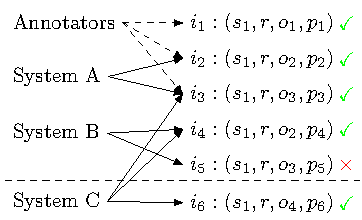
\includegraphics[width=0.9\columnwidth]{figures/pooling}
  \caption{\label{fig:pooling}
  In pooled evaluation, an evaluation dataset is constructed by labeling the relation instances collected from the pooled systems (A and B) and those identified by a team of human annotators (Annotators).
 % Arrows indicate which systems extract which relation instances.
  However, when a new system (C) is evaluated on this dataset, some of its predictions are previously unseen and can not be fairly evaluated.
  Here, the precision and recall for C should be $\frac{3}{3}$ and $\frac{3}{4}$ respectively, but its evaluation scores are estimated to be $\frac{2}{3}$ and $\frac{2}{3}$.
  The discrepancy between these two scores is called \textit{pooling bias}.
  }
\end{figure}

% 2. How is KBP evaluated? 
The primary source of evaluation data for KBP comes from the annual TAC KBP competition organized by NIST \citep{ji2011kbp}.
As mentioned earlier, the dataset is constructed by evaluating every relation instance predicted by 
the participating systems for subject entities that belong to a held-out set of evaluation entities.
%A relational tuple for the relation (\entity{Carrie Fisher}, \relation{child of}, \entity{Debbie Reynolds}) that specifies an ambiguous provenance like ``\mention{Carrie Fisher} and \mention{Debbie Reynolds} arrived together at the awards show'' would be considered incorrect.
Separately, a team of annotators identify relations for the same evaluation entities by manually searching the document corpus within a time budget.
These two sets of labeled relation instances are combined and released as the evaluation dataset.
In the example in \reffig{pooling}, systems A and B were used in constructing the pooling dataset, and there are 3 distinct relations in the dataset, between $s_1$ and $o_1$, $o_2$ and $o_3$.

A system is evaluated on the precision of its predicted relation instances for the evaluation entities and on the recall of the \textit{relations} it predicts for the same entities (see \reffig{pooling} for a worked example).
When using the evaluation data during system development, it is common practice to use the more lenient \anydoc{} score that ignores the provenance when checking if a relation instance is true.
Under this metric, predicting the relation (\entity{Carrie Fisher}, \relation{child of}, \entity{Debbie Reynolds}) from an ambiguous provenance like ``\mention{Carrie Fisher} and \mention{Debbie Reynolds} arrived together at the awards show'' would be considered correct even though it would be marked wrong under the official metric.

%$t_5$ would be considered to be correct and system B would get a precision and recall of $\frac{2}{2}$ and $\frac{2}{3}$ respectively.

% TODO: do we really need to talk about duplicates?
%\footnote{%
%  The official scoring metric also penalizes systems that predict duplicated relations (e.g.\ if they also predict (\entity{Carrie Fisher}, \relation{child of}, \entity{Debbie})); these typically arise due to an error in entity linking.
%}
%system A would get a precision of $\frac{2}{2}$ for predicting $t_2$ and $t_3$ while system B would get a precision of $\frac{1}{2}$ because $t_5$ specified an incorrect provenance.
%Recall is the fraction of true \textit{relations} that the system identifies, irrespective of which provenance it uses as long as the provenance is correct.
%Thus, system A would get a recall of $\frac{2}{3}$ while system B would only get a recall of $\frac{1}{3}$.
%Finally, \fone{} is the harmonic mean of precision and recall.

%\paragraph{Pooling bias.}
%As part of the competition, every relation predicted for the evaluation entities by the participating systems is labeled by annotators.
%However, when this dataset is used during system development, a new system (e.g.\ system C) may predict relational tuples that are not part of the dataset (e.g.\ $t_6$).
%These tuples can not be assessed without labeling the predictions and are considered to be wrong by default.
%As a result, system C would be evaluated to have a precision and recall of $\frac{2}{3}$ and $\frac{2}{3}$.
%On the other hand, if system C had participated in the pooling process, and $t_6$ were indeed correct, system C get higher precision and recall scores of $\frac{3}{3}$ and $\frac{3}{4}$ and would rank higher than system A.\footnote{Note that the recall scores of system A and B would also decrease because a new true relation had been found.}
%The discrepancy between the scores of a system because it did not participate in the pooling process is called pooling bias.

% vv OLD as of 4/8/17 

%In this section, we'll review the knowledge base population task, define appropriate notation, describe relevant evaluation metrics and discuss the standard evaluation methodology adopted by the TAC-KBP competition.
%
%\subsection{Knowledge base population}
%
%% TODO: move to a figure.
%%``[Carrie] Fisher’s mother, entertainer Debbie Reynolds, said on Twitter on Sunday that her daughter was in stable condition.''
%%Teams are then required to identify spans in the text that correspond to entities (e.g. ``\textit{Fisher}'', ``\textit{Debbie Reynolds}''),
%%assign these entities a canonical id (e.g. \texttt{Carrie\_Fisher}, \texttt{Debbie\_Reynolds})
%%  and, finally, identify all facts about mentioned entity expressed in the surrounding context (e.g. \texttt{Carrie\_Fisher per:parents Debbie\_Reynolds} or \texttt{Debbie\_Reynolds per:title entertainer}).
%
%\begin{figure}[t]
%  \centering
%%  \begin{subfigure}{0.49\textwidth}
%    [Carrie] \textbf{Fisher}’s mother, \textbf{entertainer} \textbf{Debbie Reynolds}, said on \textbf{Twitter} on \textbf{Sunday} that \textbf{her daughter} was in stable condition.
%    % TODO: example figure.
%  %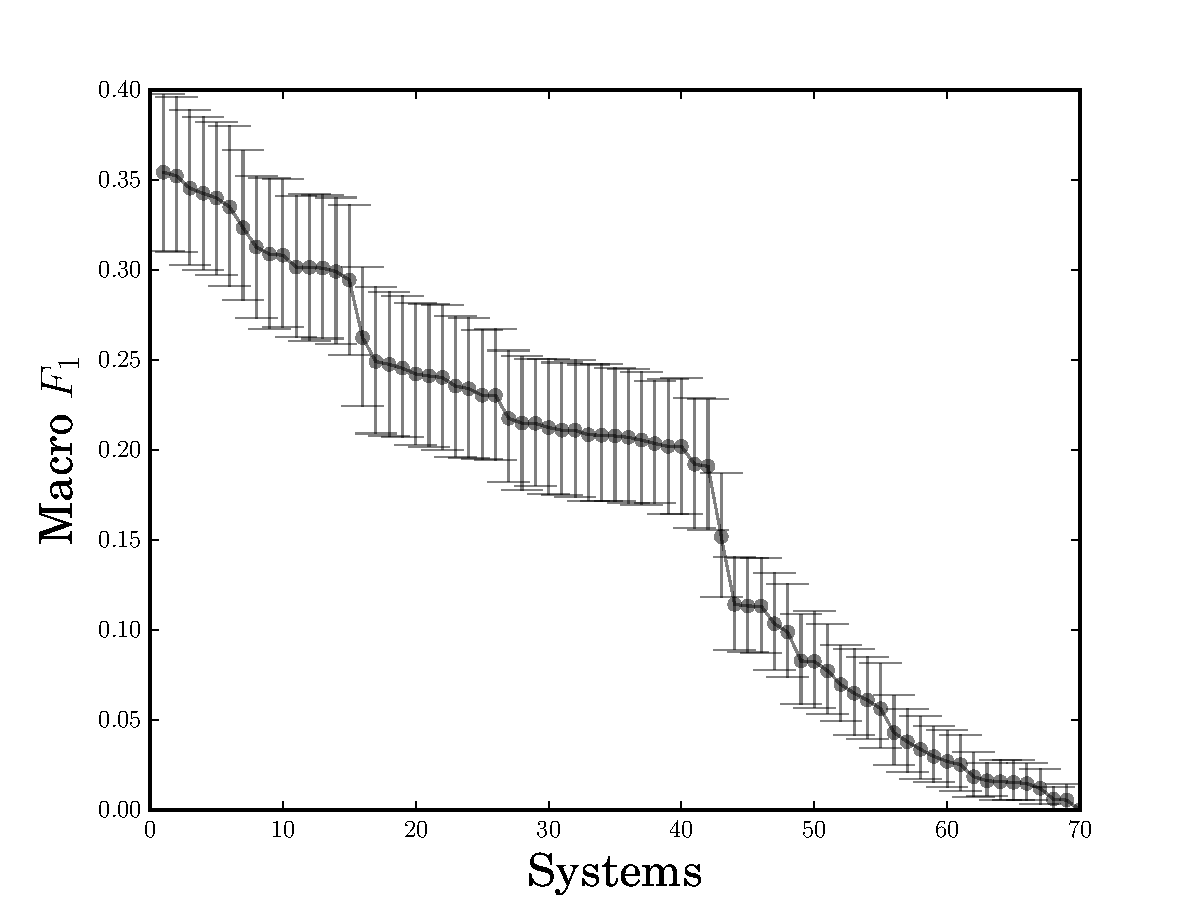
\includegraphics[width=\columnwidth]{figures/experiment1}
%%  \end{subfigure}
%%  \hfill
%%  \begin{subfigure}{0.49\textwidth}
%%  % vim:ft=tex
% Diagram depciting how mentions and entities are sampled.
\documentclass{article}
%\usetikzlibrary{...}% tikz package already loaded by 'tikz' option
\usepackage{scabby-diag}
\usepackage{booktabs}
\usetikzlibrary{fit}
\usetikzlibrary{patterns}

\begin{document}

\tikzset{correct/.style = {fill=green},
         incorrect/.style = {pattern=north east lines, pattern color=red},
         node/.style = {circle, scale=.7},
         sysa/.style = {draw, circle, dashed, thick, purple},
         sysb/.style = {draw, circle, dotted, thick, blue},
         output/.style = {inner sep=-2pt},
         duplicate/.style = {draw, rectangle, thick, red},
         part/.style = {draw, rectangle, dashed, black, thick},
        }

\begin{table}
\begin{tabular}{l | c c c c} \toprule
  $s$ & $f_1$ & $f_2$ & $f_3$ & $f_4$ \\ \midrule
  & 
    \tikz{
  \node[node,correct] (m11){$m_{11}$};
  \node[sysa,output,fit= (m11)] (m11A){};
  } 
  & 
  \tikz{
  \node[node, correct] (m21) {$m_{21}$};
    \node[sysa, output, fit= (m21)] (m21A) {};
  }
  & 
  \tikz{
    \node[node, correct] (m31) {$m_{31}$};
    \node[sysa, output, fit= (m31)] (m31A) {};
    }
  & 
  \tikz{
    \node[node, correct] (m41) {$m_{41}$};
    }
  \\

  & 
  \tikz{
  \node[node,incorrect] (m12){$m_{12}$};
  \node[sysb,output,fit= (m11)](m11B){};
  } 
  & 
  \tikz{
    \node[node, incorrect] (m22) {$m_{22}$};
    \node[sysb, output, fit= (m22)] (m22B) {};
  }
  
  &
  \tikz{
    \node[node, correct] (m32) {$m_{32}$};
    \node[sysa, output, fit= (m32)] (m32A) {};
    \node[duplicate, fit= (m32A)] (m32AD) {};
    }
  & \\
  & 
  \tikz{
    \node[node,correct] (m13){$m_{13}$};
  }
  & & & \\
  & 
    \tikz{
  \node[node,correct] (m14){$m_{14}$};
  \node[sysa,output,fit= (m14)] (m14A){};
  \node[sysb,output,fit= (m14A)]{};
  } 
  \\
  \bottomrule

\end{tabular}
\end{table}


\end{document}

%%  \end{subfigure}
%%  \caption{Evaluating KBP \pl{need more explanation}}
%\caption{\label{fig:example} An example describing entities and relations in knowledge base population.}
%\end{figure}
%
%In the knowledge base population,
% we are given a document corpus and must identify entities and relations mentioned within:
% the task is really a combination of entity detection, entity linking and relation extraction. 
%Let's start with an example to understand how entities and relations are defined: \figureref{example} discusses the late actress Carrie Fisher.
%
%Primarily, we care about named entities corresponding to people, organizations and places (formally, geo-political entities):\footnote{%
%  The most recent TAC-KBP competition also includes facilities and locations as entity types. We ignore these types in this paper.}
%this sentence mentions three entities,
%  ``\textit{Fisher}'',
%  ``\textit{Debbie Reynolds}'' and
%  ``\textit{Twitter}''.
%  Each \textit{entity mention} is also associated with a \textit{canonical entity}, described by a unique identifier, e.g.\ Wikipedia page titles. % TODO: handle NIL clusters
%In the example, the mention $m$, ``\textit{Fisher}'', is linked to the canonical entity $e$, \texttt{Carrie\_Fisher}.
%
%We also care about the \textit{relations} between entities.
%The subject of a relation is always an entity, while the object
%could be an entity, a number, a date or even an arbitrary string like ``entertainer''. 
%The sentence describes a relation $r$, \texttt{per:parents}, between the mentions $m_s$, ``\textit{Fisher}'', and $m_o$ ``\textit{Debbie Reynolds}'', and consequently a relation between the entities \texttt{Carrie\_Fisher} and \texttt{Debbie\_Reynolds}.
%We consider 39 binary relations described in the TAC-KBP specifications~\citep{ellis2015tackbp}.\footnote{%
%  There are in total 65 relations (including inverse relations) defined in the specifications.
%  We simplify the set of relations by collapsing distinct location relations like \texttt{per:city\_of\_birth} and \texttt{per:country\_of\_birth} into a single relation, \texttt{per:place\_of\_birth}.
%  We also ignore a few rare relations: \texttt{per:age}, \texttt{per:charges}, \texttt{per:cause\_of\_death} and \texttt{org:number\_of\_employees}}
%% Is this needed?
%Finally, when a system predicts a relation, it must also specify the provenance $p$ used to justify it, e.g.\ the sentence.
%
%We call the pair $(m, e)$ a \textit{link} and the tuple $(m_s, r, m_o, p)$ a \textit{relation instance}.
%Formally, the knowledge base outputted by a system consists of all the links and relation instances it could find in the corpus..
%
%%As you \pl{avoid 2nd person} can see, knowledge base population is actually composed of three tasks: entity detection, entity linking, and relation extraction.
%%This coupling allows us to aggregate facts extracted from multiple documents by the canonical entity and ask relational \pl{replace with compositional?} queries of the database so constructed, e.g.\ ``what do Carrie Fisher's parents do?''
%%Accordingly, evaluating the output of a KBP system can be defined at two levels, at the mention-level and at the entity-level.
%%Let us now see an example of how to score the output of two systems $A$ and $B$, summarized in \figureref{evaluation-table}.
%
%\subsection{Evaluation metrics}
%
%The relations predicted by a knowledge base population system can evaluated be on precision, recall and \fone{} solely at the instance-level, the relation-level or the entity-level: each of these levels describes a different type of aggregation.
%
%At the instance-level, we only evaluate whether a system has correctly predicted a relation instance $i = (m_s, r, m_o, p)$, i.e.\ whether two mentions $m_s$ and $m_o$ share a relation $r$ \textit{according the provenance $p$}, irrespective of bad linking decisions (e.g.\ linking the \textit{Fisher} in the text with the mathematician \texttt{Ronald\_Fisher}).
%If $I$ is the set of instances predicted and $I^*$ is the set of true instances in the corpus, precision and recall are simply,
%%In this example, we can compute the \textit{mention-level} precision and recall \pl{of a system $A$} as, \pl{i'd use $P^\text{m}_A$ so that $m$ doesn't seem like an unbound variable}
%\begin{align*}
%  P^\text{i} &\eqdef \frac{|I \intersection I^*|}{|I|} & %= \frac{|\{c_{11}, c_{14}, c_{21}, c_{31}, c_{32}\}|}{|\{c_{11}, c_{14}, c_{21}, c_{31}, c_{32}\}|} = 1 \\
%  R^\text{i} &\eqdef \frac{|I \intersection I^*|}{|I^*|} &
%  \fone^\text{i} &\eqdef \frac{2 P^\text{i} R^\text{i}}{P^\text{i} + R^\text{i}}.
%  %&= \frac{|\{c_{11}, c_{14}, c_{21}, c_{31}, c_{32}\}|}{|\{c_{11}, c_{14}, c_{21}, c_{31}, c_{32}, c_{13}, {c_{41}}\}|} = \frac{5}{7},
%\end{align*}
%%where $C$ is the set of all contexts predicted to contain relation returned by the system and $C^*$ are the set of all contexts that contain a relation in the corpus.
%Instance-level scores are simply macro-aggregated over each relation to get relation-level precision, recall and \fone{}, $P^\text{i}, R^\text{i}, \fone^\text{i}$.
%
%\pl{I found the text hard to understand; maybe it's better to write down the
%actual general formula?  does that look reasonable?
%Maybe a good way to visualize this as a rooted tree
%where you have the first level split on entity, the second level split on fill,
%and the third level split on instance;
%Then you can just describe entity-level scores as just different averaging at different levels of this tree
%}
%At the entity-level, instances are grouped by \textit{subject entities} and \textit{fills}, i.e.\ relation, object entity pairs, using the predicted links. Precision and recall scores are first averaged over the instances in each fill \pl{and subject, right?}, then over the fills in the subject entity and finally over all entities. For example, let $i_1, i_2, i_3, i_4$ be four relation instances for an entity $e$ where $i_1, i_2$ correspond to fill $f_1$ and $i_3, i_4$ to $f_2$. If a system predicts $I = \{i_1, i_2, i_3\}$ and $I^* = \{i_1, i_3, i_4\}$, its instance-level scores would be
%\begin{align*}
%  P^\text{i} &= \frac{|\{i_1, i_3\}|}{|\{i_1, i_2, i_3\}|} = \frac{2}{3} &
%  R^\text{i} &= \frac{|\{i_1, i_3\}|}{|\{i_1, i_3, i_4\}|} = \frac{2}{3},
%\end{align*}
%while its entity-level scores for the entity $e$ would be
%\begin{align*}
%  P^\text{e} &= \half \left(\frac{|\{i_1\}|}{|\{i_1, i_2\}|} + \frac{|\{i_3\}|}{|\{i_3\}|} \right) = \frac{3}{4} \\
%  R^\text{e} &= \half \left(\frac{|\{i_1\}|}{|\{i_1\}|} + \frac{|\{i_3\}|}{|\{i_3, i_4\}|} \right) = \frac{3}{4}.
%\end{align*}
%While both instance-level and relation-level scores are useful diagnostic metrics, entity-level scores are a better measure of performance for end applications because they measure how accurate and complete a knowledge base entry is.
%For this reason, entity-level scores are reported in the TAC-KBP evaluations.\footnote{%
%  The TAC-KBP evaluation only accepts a single relation instance per fill and hence does not need the additional step of aggregating over relation instances.
%}
%
%%\pl{clarify whether entity-level ground truth is always just a union of the mention-level ground truths? I'm guessing no}
%%At the entity-level, we focus on an entity $e_s$ and ask if the system has correctly identified a relation $r$ with another entity $e_o$ \textit{given some context $c$}, or the fill $f$.
%%Thus, system's A and B both get full credit for identifying the fill $f_1$, even though system A had found two contexts that expressed $f_1$.  
%%On the other hand, if a system falsely reports two distinct fills when there was only one, as was the case with system A and $m_{32}$, only one is considered correct, and the system loses precision for reporting an incorrect answer. 
%%Thus, the entity-level precision and recall scores are,
%%\begin{align*}
%%  P^e_A &\eqdef \frac{|F \intersection F^*|}{|F|} &= \frac{|\{f_{1}, f_{2}, f_{3}\}|}{|\{f_{1}, f_{2}, f_{3}, f_{3}'\}|} &= \frac{3}{4} \\
%%  R^e_A &\eqdef \frac{|F \intersection F^*|}{|F^*|} &= \frac{|\{f_{1}, f_{2}, f_{3}\}|}{|\{f_{1}, f_{2}, f_{3}, f_{4}\}|} &= \frac{3}{4}.
%%\end{align*}
%%where $F$ is the set of all slot fills for the entity $e$ returned by the system and $F^*$ are the set of all slot fills for the entity $e$ in the corpus.
%%
%%The entity-level metrics can be either micro or macro averaged.
%%% TODO: fix notation. handle \fone.
%%The standard metric we will be using in this paper is macro-averaged $\fone^e \eqdef \frac{1}{|E|} \sum_{e \in E} \fone^{e}$.
%%
%%\pl{the concrete example is really nice and clear;
%%I think we'll have to slim it down to make it fit (since it is pretty basic)
%%}
%
%%\paragraph{The TAC-KBP competition.}
%%% TODO provide some details about the competition -- its history. Talk about how slotfilling led to kbc.
%%%
%%
%%\paragraph{Evaluation methodology.}
%%% TODO how is the output evaluated? what are queries (how many)? how much output is evaluated? Human systems? what metrics are used (in relation to math above). Quick note about entry points and how entities are identified as being the same cluster / id as a specified entity.
%%
%%\pl{I guess defining the pooling setup formally is pretty important here}
%
%\subsection{Evaluation at TAC-KBP}
%
%The primary source of evaluation data for KBP comes from the annual TAC-KBP competition organized by NIST.\@ % TODO: add links to workshop overview papers
%Each year, participating teams submit their predicted KBs for a provided corpus.
%The organizers then use held-out relational queries that ask for relation instances that answer specific questions, e.g.\ ``where was Carrie Fisher born?'' or ``what did Carrie Fisher's parents do?'', to select which predicted relation instances to evaluate.\footnote{%
%  Prior to 2015, teams could also participate in a ``slot-filling'' track where the evaluation queries would be provided ahead of time and teams only had to submit relation instances pertaining to the query entities.}
%Independently, human annotators also search for answers to these queries and submit their results.
%The final evaluation set is thus the union of the evaluation of system predictions and a human search.
%
%While scoring a development system against this evaluation set, only relation instances that match the same set of queries are considered.
%New features in a system may allow it to predict true relations that were previously missed, while at the same predict completely new relations even for these queries that may be true or false.
%Unfortunately, there is no way to evaluate these new predictions and they are assumed false under the closed world heuristic.
%
%Another common heuristic used by teams developing systems for TAC-KBP is the \anydoc{} heuristic which treats any relation whose object string (e.g.\ ``Debbie Reynolds'' in \figureref{example}) exactly matches that of a correct relation instance in the evaluation set.
%Under this heuristic, predicting the \texttt{per:parents} relation between Carrie Fisher and Debbie Reynolds for the sentence ``\textit{Carrie Frances Fisher} was born \ldots to actors and singers Eddie Fisher and \textit{Debbie Reynolds}'' or the sentence ``Bright Lights: Starring \textit{Carrie Fisher} and \textit{Debbie Reynolds}'' would both be considered correct, even though latter is incorrect.
%
%\pl{I think a lot of this text should be replaced with a figure / simple example
%of the pooled evaluation.
%It's really important for non-KBP people to know exactly what the evaluation is doing;
%it's a simple idea, but it's too easy to gloss over the text
%}
%
%% TODO: describe `anydoc'
